\section{Experimentkonfiguration}\label{section:konzeption:experimentkonfiguration}

Die IDE soll in verschiedenen Experimentkonfigurationen nutzbar sein. In \autoref{requirement:Eigenständig nutzbar} wird verlangt, dass Experimente, welche nur die IDE als Laborgerät enthalten, ausführbar sein sollen. Weiterhin soll die IDE in Verbindung mit Steuereinheiten, wie z.B. Microcontrollern und FPGAs, genutzt werden können. Diese können wiederum mit steuerbaren Laborgeräten verbunden sein. Viele der Funktionen, die in den folgenden Abschnitten besprochen werden, sind nur in speziellen Fällen in einer eigenständigen Variante der IDE nutzbar. Weiterhin ist die Nutzung von Steuereinheiten ohne verbundene steuerbare Laborgeräte oftmals nicht zielführend. Daher wird für die folgenden Abschnitte von einem Experiment ausgegangen, welches die IDE sowie mindestens eine Steuereinheit und mindestens ein steuerbares Laborgerät enthält. Falls neue Laborgeräte oder CrossLab-Services eingeführt werden, wird deren mögliche Einbindung in die betrachtete Experimentkonfiguration beschrieben.

\begin{figure}[htbp]
    \centering
    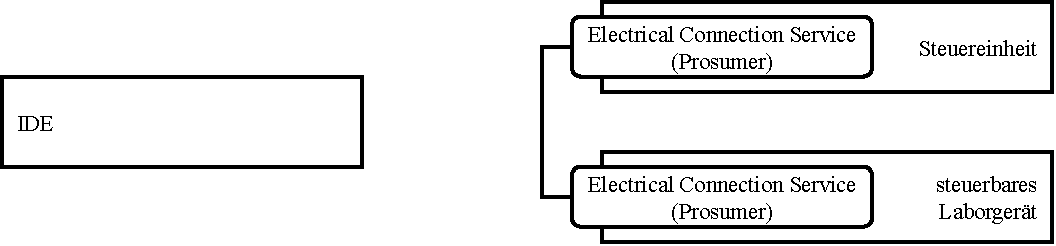
\includegraphics[width=\textwidth]{diagrams/experimentkonfigurationen/Experimentkonfiguration-00.drawio.pdf}
    \caption{Experimentkonfiguration}
    \label{figure:experimentkonfiguration:basis}
\end{figure}